% unit: u25
% sources: sources/066-differential-equations-and-exp-at.txt, sources/045-lecture-23-differential-equations-and-exp-at.txt, sources/200-mit18-06scf11-ses2-10sum-pdf-download-file.txt, sources/046-problem-solving-determinants-and-volumedifferential-equation.txt, sources/201-mit18-06scf11-ses2-10prob-pdf-download-file.txt, sources/202-mit18-06scf11-ses2-10sol-pdf-download-file.txt
\section{Differential equations and \texorpdfstring{\(e^{At}\)}{exp(At)}}\label{sec:u25}

Section~\ref{sec:u24} solved $\vb{u}_{k+1}=A\vb{u}_k$, where time moves in steps and the
solution is built from powers $\lambda^{k}$. Here time is continuous: we solve the system of
linear, constant-coefficient differential equations
\[
  \frac{d\vb{u}}{dt}=A\vb{u},\qquad \vb{u}(0)\ \text{given}.
\]
The key fact from calculus is that solutions of constant-coefficient linear equations are
exponentials. Looking for an exponential solution turns the differential equation into the
eigenvalue problem, and the whole section runs parallel to the previous one with
$e^{\lambda t}$ in place of $\lambda^{k}$.

\subsection{Pure exponential solutions}

Try $\vb{u}(t)=e^{\lambda t}\vb{x}$ with a fixed vector $\vb{x}$. Then
$d\vb{u}/dt=\lambda e^{\lambda t}\vb{x}$ while $A\vb{u}=e^{\lambda t}A\vb{x}$. These agree
for all $t$ exactly when $A\vb{x}=\lambda\vb{x}$. So every eigenvalue--eigenvector pair gives
a \emph{pure exponential solution} $e^{\lambda t}\vb{x}$, and since the equation is linear,
combinations of solutions are solutions.

\begin{theorem}[Solution by eigenvectors]\label{thm:u25-solution}
Let $A$ have $n$ independent eigenvectors $\vb{x}_1,\dots,\vb{x}_n$ with eigenvalues
$\lambda_1,\dots,\lambda_n$. Given $\vb{u}(0)$, solve $X\vb{c}=\vb{u}(0)$ for the coefficients
$c_i$. Then
\[
  \vb{u}(t)=c_1e^{\lambda_1t}\vb{x}_1+c_2e^{\lambda_2t}\vb{x}_2+\dots+c_ne^{\lambda_nt}\vb{x}_n
\]
solves $d\vb{u}/dt=A\vb{u}$ with the given initial value.
\end{theorem}

\begin{proof}
Each term satisfies the equation:
$\frac{d}{dt}\bigl(c_ie^{\lambda_it}\vb{x}_i\bigr)=c_i\lambda_ie^{\lambda_it}\vb{x}_i
=c_ie^{\lambda_it}A\vb{x}_i=A\bigl(c_ie^{\lambda_it}\vb{x}_i\bigr)$. Adding the terms, the sum
satisfies it too. At $t=0$ every exponential equals $1$, so
$\vb{u}(0)=c_1\vb{x}_1+\dots+c_n\vb{x}_n=X\vb{c}$, which is the given vector. (That this is
the \emph{only} solution follows from the matrix exponential below.)
\end{proof}

Set the two formulas side by side: $\vb{u}_k=\sum c_i\lambda_i^{k}\vb{x}_i$ for steps and
$\vb{u}(t)=\sum c_ie^{\lambda_it}\vb{x}_i$ for continuous time. Each eigenvector component
evolves on its own; $A$ couples the components of $\vb{u}$, and the eigenvectors uncouple
them.

\begin{example}[Flow between two compartments]\label{ex:u25-flow}
Solve
\[
  \frac{du_1}{dt}=-u_1+2u_2,\qquad \frac{du_2}{dt}=u_1-2u_2,\qquad \vb{u}(0)=(1,0).
\]
\emph{Eigenvalues.} $A=\left[\begin{smallmatrix} -1&2\\ 1&-2\end{smallmatrix}\right]$ is
singular (column~2 is $-2$ times column~1), so $\lambda_1=0$; the trace $-3$ gives
$\lambda_2=-3$. Directly, $\det(A-\lambda I)=\lambda^{2}+3\lambda=\lambda(\lambda+3)$.

\emph{Eigenvectors.} $A\vb{x}_1=\vb{0}$ gives $\vb{x}_1=(2,1)$.
$A+3I=\left[\begin{smallmatrix} 2&2\\ 1&1\end{smallmatrix}\right]$ gives $\vb{x}_2=(1,-1)$.

\emph{Coefficients.} $X\vb{c}=\vb{u}(0)$ reads $c_1(2,1)+c_2(1,-1)=(1,0)$; adding the
components, $3c_1=1$, and then $c_2=1-2c_1=\tfrac13$. So $c_1=c_2=\tfrac13$ and
\[
  \vb{u}(t)=\frac13\begin{bmatrix} 2\\ 1\end{bmatrix}+\frac13e^{-3t}\begin{bmatrix} 1\\ -1\end{bmatrix},
  \qquad\text{i.e.}\quad u_1=\tfrac23+\tfrac13e^{-3t},\quad u_2=\tfrac13-\tfrac13e^{-3t}.
\]
\emph{Check.} $u_1'=-e^{-3t}$ and $-u_1+2u_2=-\tfrac23-\tfrac13e^{-3t}+\tfrac23-\tfrac23e^{-3t}=-e^{-3t}$.

\emph{Interpretation.} Material flows out of compartment~1 into compartment~2. The
$e^{-3t}$ term dies out, and the $e^{0t}=1$ term stays: the solution approaches the steady
state $\vb{u}(\infty)=(\tfrac23,\tfrac13)$, the eigenvector for $\lambda=0$ scaled by $c_1$
(Figure~\ref{fig:u25-flow}). The total $u_1+u_2$ stays equal to $1$ throughout, because the
columns of $A$ add to zero, so $\frac{d}{dt}(u_1+u_2)=0$.
\end{example}

\begin{figure}[ht]\centering
\begin{tikzpicture}
\begin{axis}[width=0.6\textwidth,height=0.36\textwidth,xmin=0,xmax=2,ymin=0,ymax=1.05,
  xlabel={$t$},ylabel={$u_i(t)$},axis lines=left,ytick={0,0.3333,0.6667,1},
  yticklabels={$0$,$\tfrac13$,$\tfrac23$,$1$},
  every axis plot/.append style={thick,samples=80}]
  \addplot[gray,dashed,domain=0:2] {2/3};
  \addplot[gray,dashed,domain=0:2] {1/3};
  \addplot[blue,domain=0:2] {2/3+exp(-3*x)/3} node[pos=0.12,above right] {$u_1(t)$};
  \addplot[red!80!black,domain=0:2] {1/3-exp(-3*x)/3} node[pos=0.12,below right] {$u_2(t)$};
\end{axis}
\end{tikzpicture}
\caption{The solution $u_1=\tfrac23+\tfrac13e^{-3t}$, $u_2=\tfrac13-\tfrac13e^{-3t}$ of
Example~\ref{ex:u25-flow}. The eigenvalue $\lambda_2=-3$ makes the
difference from the steady state decay like $e^{-3t}$ (by $t=1$ only $5\%$ of it is left);
the eigenvalue $\lambda_1=0$ supplies the steady state $(\tfrac23,\tfrac13)$.}
\label{fig:u25-flow}
\end{figure}

\subsection{Stability and steady states}

Which way the solution goes is decided by the eigenvalues alone. For a complex eigenvalue
$\lambda=a+ib$,
\[
  e^{\lambda t}=e^{at}e^{ibt}=e^{at}(\cos bt+i\sin bt),\qquad |e^{\lambda t}|=e^{at},
\]
since $\cos^{2}bt+\sin^{2}bt=1$. The imaginary part only makes the solution oscillate; the
real part decides growth or decay. For instance $\lambda=-3+6i$ gives $|e^{\lambda t}|=e^{-3t}$.
For a diagonalizable $A$, Theorem~\ref{thm:u25-solution} therefore gives three regimes:
\begin{enumerate}
  \item \emph{Stability}: $\vb{u}(t)\to\vb{0}$ for every start exactly when
  $\operatorname{Re}\lambda_i<0$ for every $i$.
  \item \emph{Steady state}: if $\lambda_1=0$ and all other $\operatorname{Re}\lambda_i<0$,
  then $\vb{u}(t)\to c_1\vb{x}_1$.
  \item \emph{Blow-up}: if some $\operatorname{Re}\lambda_i>0$, every start with $c_i\neq0$
  produces a solution that grows without bound.
\end{enumerate}
Changing $A$ to $-A$ changes the sign of every eigenvalue: in Example~\ref{ex:u25-flow} it
would turn $e^{-3t}$ into $e^{3t}$ and the steady state into blow-up.

\begin{figure}[ht]\centering
\begin{tikzpicture}[scale=0.85,>=Stealth]
  \fill[blue!10] (-2.6,-2.2) rectangle (0,2.2);
  \draw[->] (-2.7,0) -- (2.7,0) node[right] {$\operatorname{Re}\lambda$};
  \draw[->] (0,-2.3) -- (0,2.4) node[above] {$\operatorname{Im}\lambda$};
  \node[blue!60!black,align=center] at (-1.3,1.7) {\small $e^{At}\to0$\\[-1pt]\small $\operatorname{Re}\lambda<0$};
  \fill (-1.2,0.8) circle (1.5pt); \fill (-1.2,-0.8) circle (1.5pt);
  \node[left] at (-1.2,-0.8) {\small $a-ib$}; \node[left] at (-1.2,0.8) {\small $a+ib$};
  \node at (0,-2.75) {differential equations};
\end{tikzpicture}\qquad
\begin{tikzpicture}[scale=0.85,>=Stealth]
  \fill[orange!15] (0,0) circle (1.5);
  \draw[orange!80!black] (0,0) circle (1.5);
  \draw[->] (-2.7,0) -- (2.7,0) node[right] {$\operatorname{Re}\lambda$};
  \draw[->] (0,-2.3) -- (0,2.4) node[above] {$\operatorname{Im}\lambda$};
  \node[orange!60!black,align=center] at (1.6,1.75) {\small $A^{k}\to0$\\[-1pt]\small $|\lambda|<1$};
  \node[below right] at (1.5,0) {\small $1$};
  \node at (0,-2.75) {difference equations};
\end{tikzpicture}
\caption{Where the eigenvalues must lie for the solutions to decay. For
$d\vb{u}/dt=A\vb{u}$ it is the left half-plane $\operatorname{Re}\lambda<0$; for
$\vb{u}_{k+1}=A\vb{u}_k$ it is the inside of the unit circle $|\lambda|<1$. The eigenvalue
$\lambda=0$ gives a steady state for differential equations; $\lambda=1$ gives one for powers.}
\label{fig:u25-regions}
\end{figure}

For $2\times2$ matrices there is a test that needs no eigenvalues at all.

\begin{proposition}[Stability of a $2\times2$ system]\label{prop:u25-2by2}
A real $2\times2$ matrix $A$ has both eigenvalues with negative real part if and only if
\[
  \tr A<0\qquad\text{and}\qquad\det A>0 .
\]
\end{proposition}

\begin{proof}
Recall $\tr A=\lambda_1+\lambda_2$ and $\det A=\lambda_1\lambda_2$
(Section~\ref{sec:u23}). If the eigenvalues are a complex pair $a\pm ib$ ($b\neq0$),
then $\tr A=2a$ and $\det A=a^{2}+b^{2}>0$, so the condition says exactly $a<0$. If they are
real, $\det A>0$ means they have the same sign and $\tr A<0$ means that sign is negative;
conversely two negative numbers have negative sum and positive product.
\end{proof}

A negative trace alone is not enough: $\left[\begin{smallmatrix} -2&0\\ 0&1\end{smallmatrix}\right]$
has trace $-1$ but eigenvalues $-2$ and $1$, so $e^{t}$ blows up. Its determinant $-2$ fails
the test.

\subsection{The matrix exponential}

For a single equation $du/dt=au$ the solution is $u(t)=e^{at}u(0)$. We would like to write
$\vb{u}(t)=e^{At}\vb{u}(0)$ for systems. The exponential of a matrix is defined by the same
power series as $e^{x}$.

\begin{definition}[Matrix exponential]\label{def:u25-exp}
For a square matrix $A$ and a number $t$,
\[
  e^{At}=I+At+\frac{(At)^{2}}{2!}+\frac{(At)^{3}}{3!}+\dots=\sum_{k=0}^{\infty}\frac{(At)^{k}}{k!}.
\]
\end{definition}

The series always converges: if every entry of $A$ has absolute value at most $m$, every entry
of $A^{k}$ has absolute value at most $(nm)^{k}$, and $\sum (nm|t|)^{k}/k!$ is finite. Compare
the geometric series $(I-At)^{-1}=I+At+(At)^{2}+\cdots$, which has no factorials and converges
only when the eigenvalues of $At$ are smaller than $1$ in absolute value; for small $t$ it says
$(I-At)^{-1}\approx I+At$.

\begin{proposition}[The exponential solves the system]\label{prop:u25-derivative}
$\dfrac{d}{dt}e^{At}=Ae^{At}$ and $e^{A\cdot0}=I$. Hence $\vb{u}(t)=e^{At}\vb{u}(0)$ solves
$d\vb{u}/dt=A\vb{u}$ with the given $\vb{u}(0)$.
\end{proposition}

\begin{proof}
Differentiate the series term by term (allowed for power series):
$\frac{d}{dt}\frac{t^{k}A^{k}}{k!}=\frac{t^{k-1}A^{k}}{(k-1)!}=A\,\frac{(At)^{k-1}}{(k-1)!}$.
Summing over $k\ge1$ gives $A\,e^{At}$. At $t=0$ only the term $I$ survives.
\end{proof}

The formula needs no eigenvectors, so it also covers matrices that are not diagonalizable.
It also gives uniqueness: if $\vb{u}$ is any solution, then
$\frac{d}{dt}\bigl(e^{-At}\vb{u}\bigr)=-Ae^{-At}\vb{u}+e^{-At}A\vb{u}=\vb{0}$ (the series show that
$A$ commutes with $e^{-At}$), so $e^{-At}\vb{u}(t)$ is constant, equal to $\vb{u}(0)$. And
$e^{At}e^{-At}=I$, because this product has derivative $Ae^{At}e^{-At}-e^{At}Ae^{-At}=0$ and
equals $I$ at $t=0$; multiplying by $e^{At}$ gives $\vb{u}(t)=e^{At}\vb{u}(0)$. When $A$ \emph{is} diagonalizable, the
eigenvectors make the series easy to sum.

\begin{theorem}[Exponential by diagonalization]\label{thm:u25-diagexp}
If $A=X\Lambda X^{-1}$, then
\[
  e^{At}=Xe^{\Lambda t}X^{-1},\qquad
  e^{\Lambda t}=\begin{bmatrix} e^{\lambda_1t} & & \\ & \ddots & \\ & & e^{\lambda_nt}\end{bmatrix}.
\]
\end{theorem}

\begin{proof}
As in Section~\ref{sec:u24}, $(At)^{k}=X\Lambda^{k}X^{-1}t^{k}$. Write $I=XX^{-1}$ and
factor $X$ out on the left and $X^{-1}$ on the right of every term:
\[
  e^{At}=X\Bigl(I+\Lambda t+\frac{(\Lambda t)^{2}}{2!}+\cdots\Bigr)X^{-1}=Xe^{\Lambda t}X^{-1}.
\]
The series for the diagonal matrix $\Lambda t$ is diagonal, with the scalar series
$\sum(\lambda_it)^{k}/k!=e^{\lambda_it}$ on the diagonal.
\end{proof}

Another way to see the same thing: substitute $\vb{u}=X\vb{v}$. Then $X\,d\vb{v}/dt=AX\vb{v}$,
so $d\vb{v}/dt=X^{-1}AX\vb{v}=\Lambda\vb{v}$, which is $n$ separate scalar equations
$dv_i/dt=\lambda_iv_i$ with solutions $v_i(t)=e^{\lambda_it}v_i(0)$. Going back,
$\vb{u}(t)=Xe^{\Lambda t}X^{-1}\vb{u}(0)$, and with $\vb{c}=X^{-1}\vb{u}(0)$ this is the sum
in Theorem~\ref{thm:u25-solution}. It also shows again that $e^{At}\to0$ exactly when every
$e^{\lambda_it}\to0$, that is, every $\operatorname{Re}\lambda_i<0$.

\begin{example}[Computing $e^{At}$]\label{ex:u25-exp}
Let $A=\begin{bmatrix} 1&1\\ 0&3\end{bmatrix}$. It is triangular: $\lambda_1=1$ with
$\vb{x}_1=(1,0)$, and $\lambda_2=3$ with $\vb{x}_2=(1,2)$ from
$A-3I=\left[\begin{smallmatrix} -2&1\\ 0&0\end{smallmatrix}\right]$. So
\[
  X=\begin{bmatrix} 1&1\\ 0&2\end{bmatrix},\qquad
  X^{-1}=\begin{bmatrix} 1&-\tfrac12\\ 0&\tfrac12\end{bmatrix},\qquad
  e^{At}=\begin{bmatrix} 1&1\\ 0&2\end{bmatrix}
  \begin{bmatrix} e^{t}&0\\ 0&e^{3t}\end{bmatrix}
  \begin{bmatrix} 1&-\tfrac12\\ 0&\tfrac12\end{bmatrix}
  =\begin{bmatrix} e^{t} & \tfrac12(e^{3t}-e^{t})\\ 0 & e^{3t}\end{bmatrix}.
\]
Check: at $t=0$ this is $I$. Its derivative is
$\left[\begin{smallmatrix} e^{t} & \frac12(3e^{3t}-e^{t})\\ 0 & 3e^{3t}\end{smallmatrix}\right]$,
which at $t=0$ equals $\left[\begin{smallmatrix} 1&1\\ 0&3\end{smallmatrix}\right]=A$, as
Proposition~\ref{prop:u25-derivative} requires.
\end{example}

\begin{trap}
The exponential of a matrix is \emph{not} the matrix of exponentials of its entries. In
Example~\ref{ex:u25-exp} the $(1,2)$ entry of $e^{At}$ is $\tfrac12(e^{3t}-e^{t})$, not
$e^{t}$, and the zero entry gives $0$, not $e^{0}=1$. Similarly $e^{A}e^{B}=e^{A+B}$ is true
when $AB=BA$ but false in general. When $A$ cannot be diagonalized, new kinds of terms
appear: for $A=\left[\begin{smallmatrix} 0&1\\ 0&0\end{smallmatrix}\right]$ we have $A^{2}=0$,
the series stops, and $e^{At}=I+At=\left[\begin{smallmatrix} 1&t\\ 0&1\end{smallmatrix}\right]$
contains $t\,e^{0t}$, which is not a pure exponential.
\end{trap}

\subsection{Higher-order equations become first-order systems}

The second-order equation $y''+by'+ky=0$ becomes a $2\times2$ system by the same trick as
for Fibonacci: take $\vb{u}=(y',y)$ and add the trivial equation $y'=y'$,
\[
  \vb{u}'=\begin{bmatrix} y''\\ y'\end{bmatrix}
  =\begin{bmatrix} -b&-k\\ 1&0\end{bmatrix}\begin{bmatrix} y'\\ y\end{bmatrix}.
\]
Its characteristic polynomial is
$\det\left[\begin{smallmatrix} -b-\lambda & -k\\ 1 & -\lambda\end{smallmatrix}\right]
=\lambda^{2}+b\lambda+k$, exactly what we get by substituting $y=e^{\lambda t}$ into the
original equation. An equation of order $m$ gives an $m\times m$ matrix with the
coefficients (with signs changed) across the first row, $1$'s just below the diagonal, and
zeros elsewhere. For such a matrix the vector $(\lambda^{m-1},\dots,\lambda,1)$ is an
eigenvector whenever $\lambda$ is an eigenvalue: the rows below the first just say
$\lambda^{j}=\lambda\cdot\lambda^{j-1}$, and the first row is the characteristic equation.

\begin{example}[A third-order equation]\label{ex:u25-third}
Solve $y'''+2y''-y'-2y=0$ and find the first column of $e^{At}$ for the corresponding
system.

With $\vb{u}=(y'',y',y)$, the equation $y'''=-2y''+y'+2y$ gives
\[
  \vb{u}'=A\vb{u},\qquad A=\begin{bmatrix} -2&1&2\\ 1&0&0\\ 0&1&0\end{bmatrix}.
\]
Expanding along the first row,
\[
  \det(A-\lambda I)=(-2-\lambda)\lambda^{2}-1\cdot(-\lambda)+2\cdot1
  =-(\lambda^{3}+2\lambda^{2}-\lambda-2)=-(\lambda-1)(\lambda+1)(\lambda+2),
\]
so $\lambda=1,-1,-2$, with eigenvectors $(\lambda^{2},\lambda,1)$:
$\vb{x}_1=(1,1,1)$, $\vb{x}_2=(1,-1,1)$, $\vb{x}_3=(4,-2,1)$. The last component of
$\vb{u}(t)=C_1e^{t}\vb{x}_1+C_2e^{-t}\vb{x}_2+C_3e^{-2t}\vb{x}_3$ is
\[
  y(t)=C_1e^{t}+C_2e^{-t}+C_3e^{-2t}.
\]
Because $\lambda=1>0$, solutions blow up unless $C_1=0$.

To get the first column of $e^{At}=Xe^{\Lambda t}X^{-1}$, only the first column of
$X^{-1}$ is needed. By the cofactor formula of Section~\ref{sec:u22} ($X^{-1}$ is the transposed cofactor matrix divided by $\det X$), that column is the cofactors of the
first row of $X$ divided by $\det X$. For
$X=\left[\begin{smallmatrix} 1&1&4\\ 1&-1&-2\\ 1&1&1\end{smallmatrix}\right]$ the cofactors
of the first row are
\[
  C_{11}=(-1)(1)-(-2)(1)=1,\qquad C_{12}=-\bigl(1\cdot1-(-2)\cdot1\bigr)=-3,\qquad
  C_{13}=1\cdot1-(-1)\cdot1=2,
\]
and $\det X=1\cdot1+1\cdot(-3)+4\cdot2=6$. So the first column of $X^{-1}$ is
$(\tfrac16,-\tfrac12,\tfrac13)$, and the first column of $e^{At}$ is
\[
  \tfrac16e^{t}\,\vb{x}_1-\tfrac12e^{-t}\,\vb{x}_2+\tfrac13e^{-2t}\,\vb{x}_3 .
\]
At $t=0$ it equals $\tfrac16(1,1,1)-\tfrac12(1,-1,1)+\tfrac13(4,-2,1)=(1,0,0)$, the first
column of $I$, as it must.
\end{example}

\subsection{Exercises}

\begin{exercise}[Skew-symmetric systems conserve length]\label{exr:u25-skew}
The matrix in
\[
  \frac{d\vb{u}}{dt}=\begin{bmatrix} 0&c&-b\\ -c&0&a\\ b&-a&0\end{bmatrix}\vb{u},
  \quad\text{that is,}\quad u_1'=cu_2-bu_3,\ \ u_2'=au_3-cu_1,\ \ u_3'=bu_1-au_2,
\]
is skew-symmetric ($A\T=-A$). Compute
$\frac{d}{dt}\|\vb{u}(t)\|^{2}$. What does this say about $\vb{u}(t)$?
\end{exercise}
\begin{solution}
\[
  \frac{d}{dt}(u_1^{2}+u_2^{2}+u_3^{2})=2u_1u_1'+2u_2u_2'+2u_3u_3'
  =2u_1(cu_2-bu_3)+2u_2(au_3-cu_1)+2u_3(bu_1-au_2)=0,
\]
since the six products cancel in pairs. So $\|\vb{u}(t)\|=\|\vb{u}(0)\|$ for all $t$: the
solution stays on the sphere of radius $\|\vb{u}(0)\|$, neither decaying nor blowing up. In
matrix form, $\frac{d}{dt}\vb{u}\T\vb{u}=\vb{u}\T(A\T+A)\vb{u}=0$ because $A\T=-A$.
Consistently, the eigenvalues of a real skew-symmetric matrix are purely imaginary
(Section~\ref{sec:u23}).
\end{solution}

\begin{exercise}[The exponential of a rotation generator]\label{exr:u25-rotation}
For $A=\left[\begin{smallmatrix} 0&-1\\ 1&0\end{smallmatrix}\right]$ show that
$e^{At}=\left[\begin{smallmatrix} \cos t & -\sin t\\ \sin t & \cos t\end{smallmatrix}\right]$.
Describe the solutions of $d\vb{u}/dt=A\vb{u}$.
\end{exercise}
\begin{solution}
$A^{2}=-I$, so $A^{3}=-A$, $A^{4}=I$, and the powers repeat with period $4$. Group the series:
\[
  e^{At}=\Bigl(1-\frac{t^{2}}{2!}+\frac{t^{4}}{4!}-\cdots\Bigr)I+\Bigl(t-\frac{t^{3}}{3!}+\cdots\Bigr)A
  =(\cos t)\,I+(\sin t)\,A,
\]
which is the stated rotation matrix. (Equivalently, the eigenvalues are $\pm i$ and
$e^{\pm it}=\cos t\pm i\sin t$.) Every solution $\vb{u}(t)=e^{At}\vb{u}(0)$ rotates
$\vb{u}(0)$ through the angle $t$: it circles the origin at constant length, the case
$\operatorname{Re}\lambda=0$ between decay and blow-up.
\end{solution}

\begin{exercise}[Stability by trace and determinant]\label{exr:u25-classify}
Decide whether solutions of $d\vb{u}/dt=A\vb{u}$ decay, blow up, or neither, for
\[
  \text{(a)}\ \begin{bmatrix} -1&5\\ -1&-1\end{bmatrix},\quad
  \text{(b)}\ \begin{bmatrix} -3&1\\ 1&-3\end{bmatrix},\quad
  \text{(c)}\ \begin{bmatrix} 0&1\\ -4&0\end{bmatrix},\quad
  \text{(d)}\ \begin{bmatrix} 1&2\\ 3&4\end{bmatrix}.
\]
\end{exercise}
\begin{solution}
Use Proposition~\ref{prop:u25-2by2}.
(a) $\tr=-2<0$, $\det=1+5=6>0$: stable. The eigenvalues are $-1\pm i\sqrt5$, so solutions
spiral into the origin.
(b) $\tr=-6$, $\det=9-1=8$: stable, with real eigenvalues $-2$ and $-4$.
(c) $\tr=0$, $\det=4$: the eigenvalues are $\pm2i$, with real part $0$. Solutions oscillate
like $\cos2t$ and $\sin2t$ forever, neither decaying nor growing. (This is $y''+4y=0$
written as a system for $(y,y')$.)
(d) $\tr=5$, $\det=4-6=-2<0$: one positive and one negative eigenvalue,
$\tfrac12(5\pm\sqrt{33})$, so solutions blow up except along one eigenvector line.
\end{solution}

\begin{exercise}[A damped oscillator]\label{exr:u25-damped}
Solve $y''+3y'+2y=0$ with $y(0)=1$, $y'(0)=0$ by writing it as a system for
$\vb{u}=(y',y)$.
\end{exercise}
\begin{solution}
$A=\left[\begin{smallmatrix} -3&-2\\ 1&0\end{smallmatrix}\right]$ and
$\det(A-\lambda I)=\lambda^{2}+3\lambda+2=(\lambda+1)(\lambda+2)$. The eigenvectors are
$(\lambda,1)$: $\vb{x}_1=(-1,1)$ for $\lambda=-1$ and $\vb{x}_2=(-2,1)$ for $\lambda=-2$.
The start $\vb{u}(0)=(y'(0),y(0))=(0,1)=c_1(-1,1)+c_2(-2,1)$ gives $-c_1-2c_2=0$ and
$c_1+c_2=1$, so $c_2=-1$, $c_1=2$. The second component of
$\vb{u}(t)=2e^{-t}\vb{x}_1-e^{-2t}\vb{x}_2$ is
\[
  y(t)=2e^{-t}-e^{-2t}.
\]
Check: $y(0)=1$, $y'(t)=-2e^{-t}+2e^{-2t}$ so $y'(0)=0$, and
$y''+3y'+2y=(2e^{-t}-4e^{-2t})+(-6e^{-t}+6e^{-2t})+(4e^{-t}-2e^{-2t})=0$. Both eigenvalues
are negative (trace $-3$, determinant $2$), so $y\to0$ without oscillating.
\end{solution}
